% FONTE TEMA https://github.com/matze/mtheme
\documentclass[aspectratio=1610]{beamer}
%\documentclass[aspectratio=1610, handout]{beamer}
\usepackage[utf8]{inputenc}
\usepackage{ragged2e}
\usepackage{xcolor}
\usepackage[italian]{babel}
\usepackage{multirow}
\usepackage{silence}
\WarningFilter{beamer}{}
\WarningFilter{metropolis}{}
\usetheme[progressbar=frametitle,titleformat=smallcaps]{metropolis}
\setbeamertemplate{frame numbering}[fraction]
\setbeamercovered{dynamic}
\definecolor{rosso}{RGB}{255, 0, 0}
\definecolor{giallo}{RGB}{254,212,23}
\hypersetup{colorlinks=true,linkcolor=black,urlcolor=rosso}
\setbeamercolor{palette primary}{fg=black, bg=giallo}
\setbeamercolor{background canvas}{bg=white}
\setbeamercolor{normal text}{fg=black}
\setbeamercolor{progress bar}{fg=rosso}
\setbeamercolor{framesubtitle}{fg=rosso}
\setbeamercolor{normal text .dimmed}{fg=giallo}
\setbeamercolor{block title alerted}{fg=rosso, bg=giallo}
\setbeamerfont{caption}{size=\tiny}
\setbeamerfont{caption name}{size=\tiny}
\setlength{\abovecaptionskip}{0pt}
\makeatletter
\metroset{block=fill}
\setlength{\metropolis@progressinheadfoot@linewidth}{1pt} 
\setlength{\metropolis@progressonsectionpage@linewidth}{1pt}
\setlength{\metropolis@titleseparator@linewidth}{1pt}
\makeatother

\title{MEMORIA E BIT}
\subtitle{Tensione e Transistor}
\date{}
\institute{\textit{
        Fonti:
        \begin{itemize}
            \item[-] \href{https://www.geopop.it/qual-e-la-differenza-tra-corrente-e-tensione/}{Geopop}
            \item[-] \href{https://www.fastweb.it/fastweb-plus/digital-magazine/com-e-fatto-e-come-funziona-un-transistor/}{Fastweb Plus}
        \end{itemize}
    }
}

\begin{document}

\begin{frame}[plain, noframenumbering]
    \titlepage
\end{frame}

\section{DEFINIZIONI}

\begin{frame}{TENSIONE ELETTRICA}
    \begin{columns}
        \column{.5\textwidth}
           \begin{alertblock}{DEFINIZIONE}
                \begin{minipage}{0.96\linewidth}
                    \justifying
                    La \textbf{tensione elettrica}, misurata in \textbf{volt (V)}, è la \textbf{differenza di 
                    potenziale elettrico} tra due punti di un circuito, ovvero \textbf{la forza che 
                    spinge gli elettroni} (le cariche elettriche) attraverso un circuito. 
                    Senza tensione non ci sarebbe movimento di cariche elettriche e quindi 
                    nessuna corrente.
                \end{minipage}
           \end{alertblock}
        \column{.5\textwidth}
            \begin{figure}
                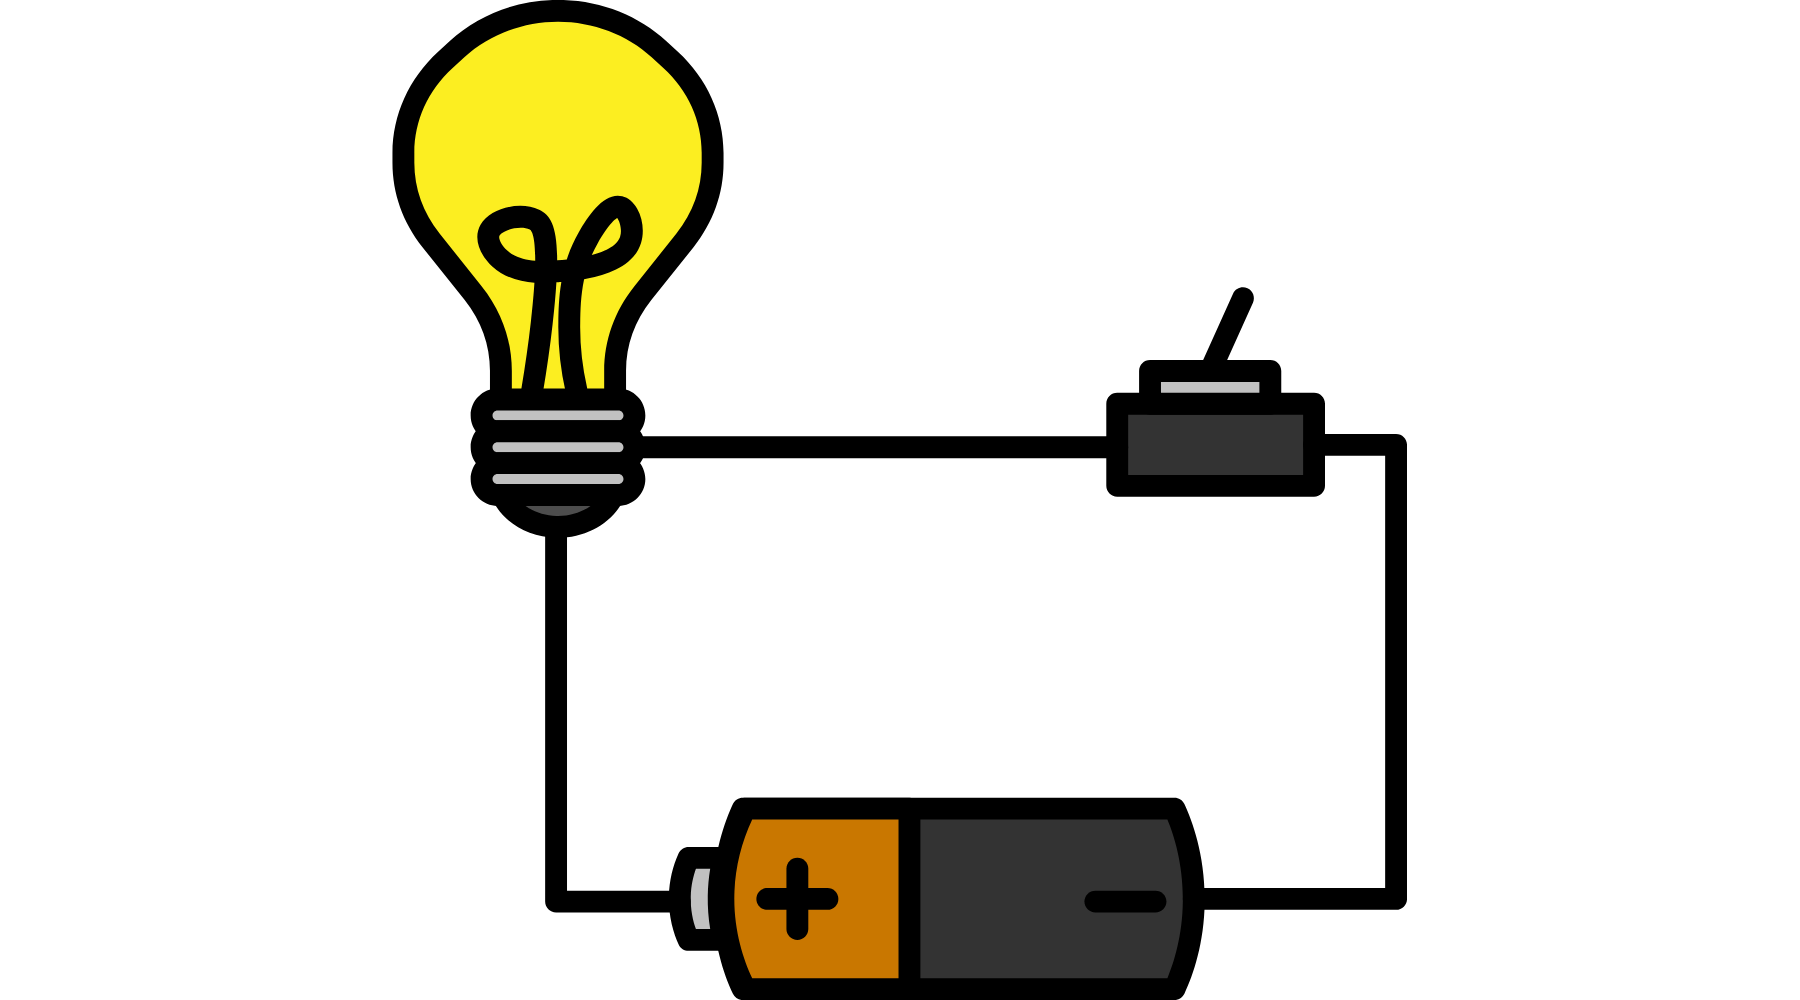
\includegraphics[width=\linewidth]{img/tensione.png}
                \caption{{creata con \href{www.canva.com}{Canva}}}
            \end{figure}
    \end{columns}
\end{frame}

\begin{frame}{TRANSISTOR}
    \begin{columns}
        \column{.6\textwidth}
           \begin{alertblock}{DEFINIZIONE}
                \begin{minipage}{0.96\linewidth}
                    \justifying
                    Il \textbf{transistor}, è un componente elettronico realizzato 
                    con diversi materiali semiconduttori (\textbf{silicio}). 
                    Al corpo del transistor sono collegati \textbf{tre terminali} utilizzati 
                    per connettere il dispositivo al circuito esterno. \textbf{Applicando una tensione 
                    elettrica} a due dei terminali è possibile regolare il flusso di elettroni 
                    che attraversa il transistor stesso, potendo così:
                    \begin{enumerate}
                        \item amplificare il segnale in ingresso 
                        (corrente elettrica in uscita superiore a quella in entrata);
                        \item utilizzarlo come \textbf{interruttore per accendere o spegnere} un circuito.
                    \end{enumerate}
                \end{minipage}
           \end{alertblock}
        \column{.4\textwidth}
            \begin{figure}
                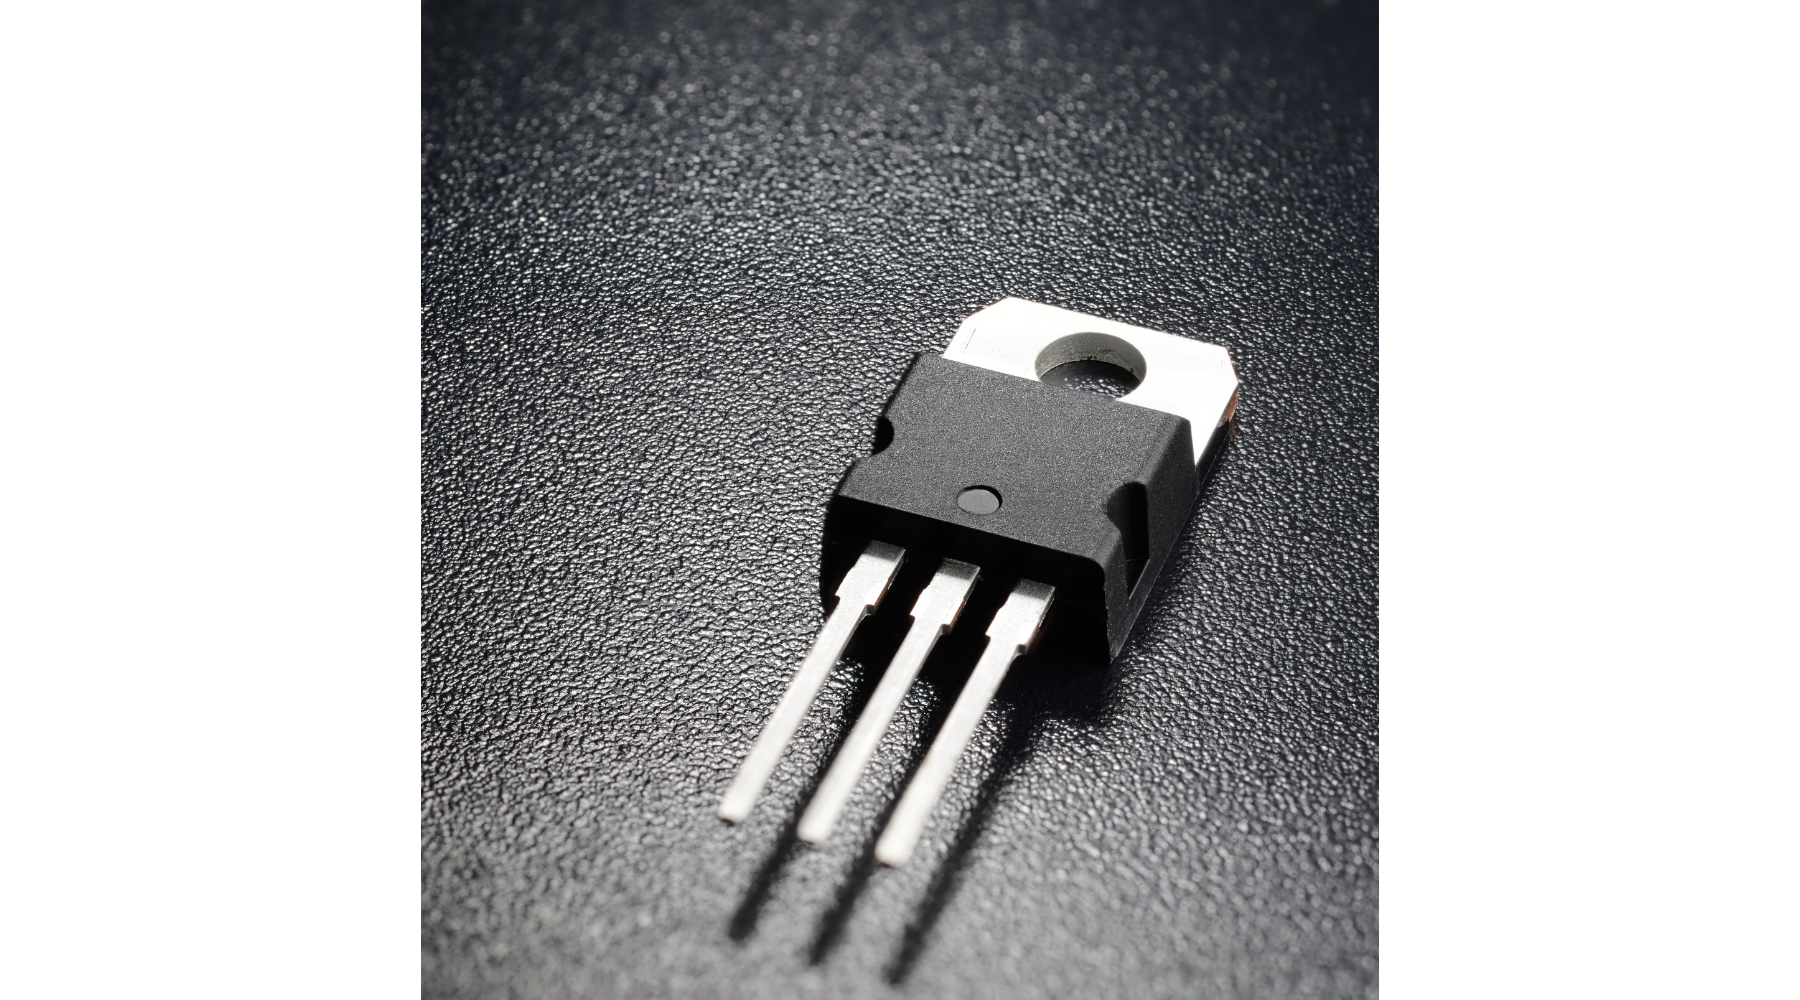
\includegraphics[width=\linewidth]{img/transistor.png}
                \caption{{creata con \href{www.canva.com}{Canva}}}
            \end{figure}
            \tiny{\textbf{Approfondimenti}}
            \begin{itemize}
                \item \tiny{\href{https://www.youtube.com/watch?v=RjHoSgWY3EA}{Funzionamento del transistor MOSFET}}
                \item \tiny{\href{https://www.geopop.it/processori-a-3-nanometri-cosa-sono-e-perche-sono-una-rivoluzione/}{Dimensioni dei transistor}}
                \item \tiny{\href{https://www.geopop.it/addio-a-gordon-moore-chi-era-lideatore-della-legge-sui-transistor-e-co-fondatore-di-intel/}{Gordon Moore e la prima legge di Moore}} 
            \end{itemize}        
    \end{columns}
\end{frame}

\section{MEMORIA E BIT}

\begin{frame}{MEMORIA E BINARIO}
    \only<1 | handout:0>{\begin{figure}
        
\includegraphics[width=\linewidth]{img/1.png}
        \caption{{creata con \href{www.canva.com}{Canva}}}
    \end{figure}}
    \only<2 | handout:1>{\begin{figure}
        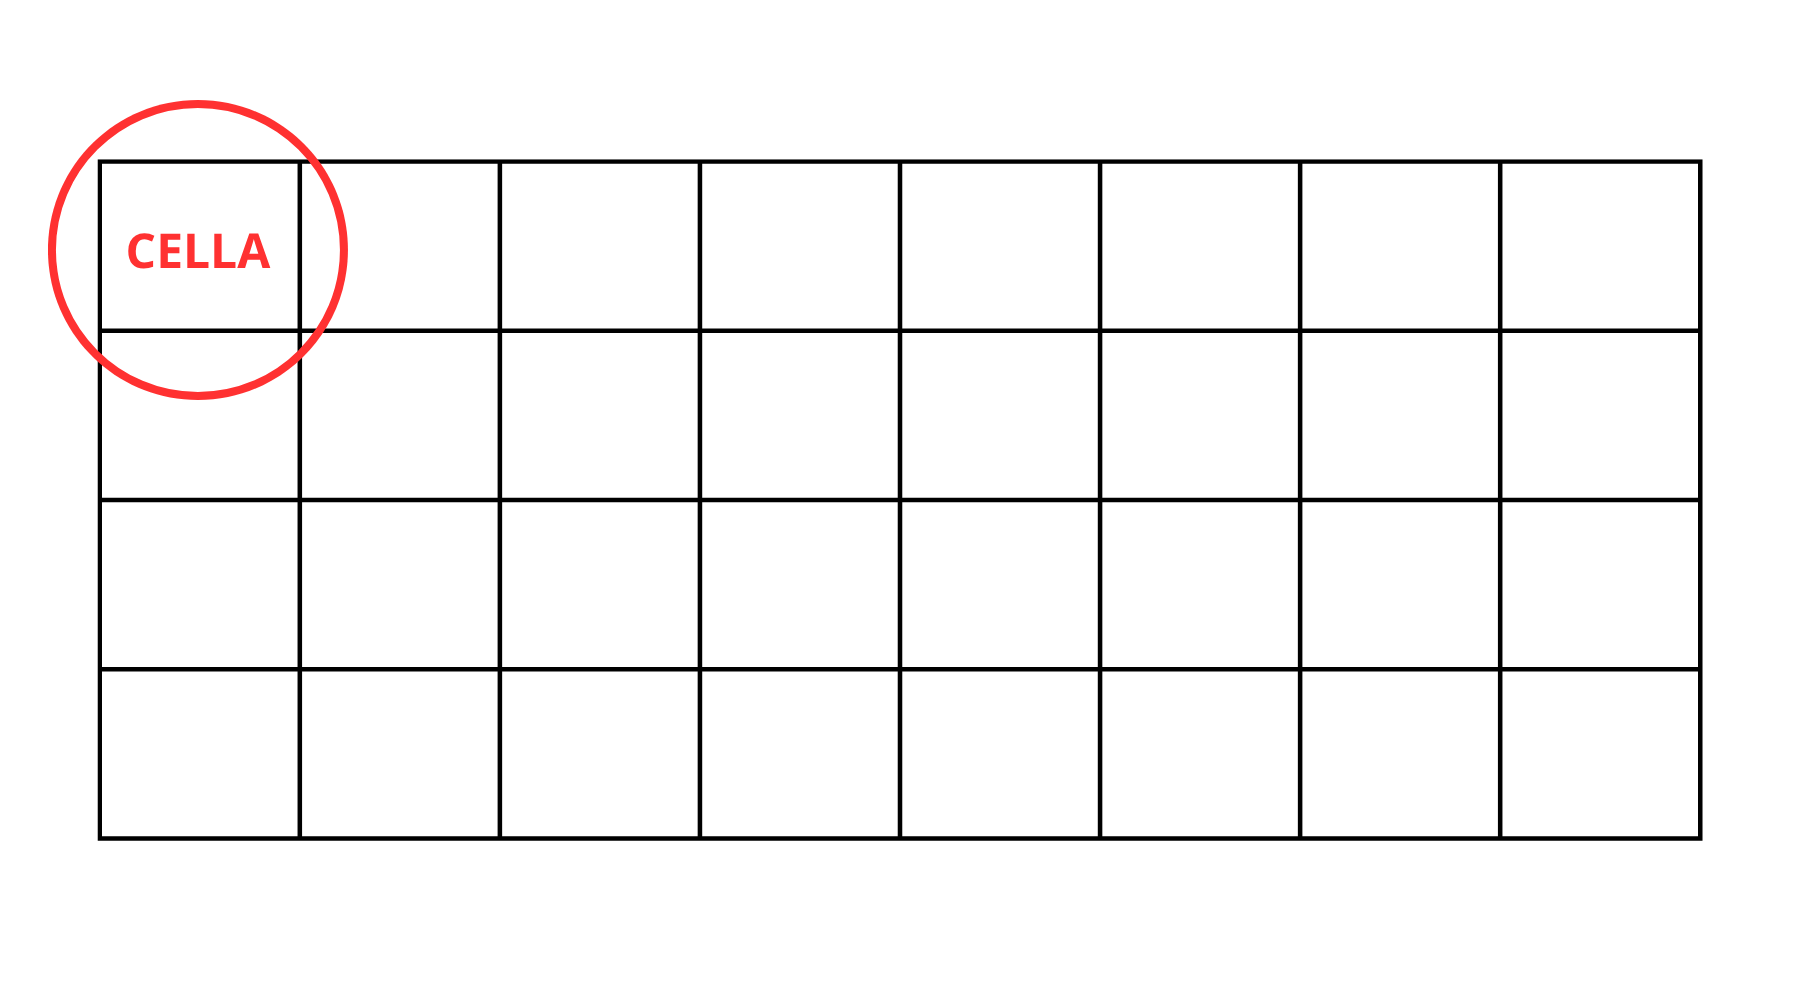
\includegraphics[width=\linewidth]{img/2.png}
        \caption{{creata con \href{www.canva.com}{Canva}}}
    \end{figure}}
    \only<3 | handout:2>{\begin{figure}
        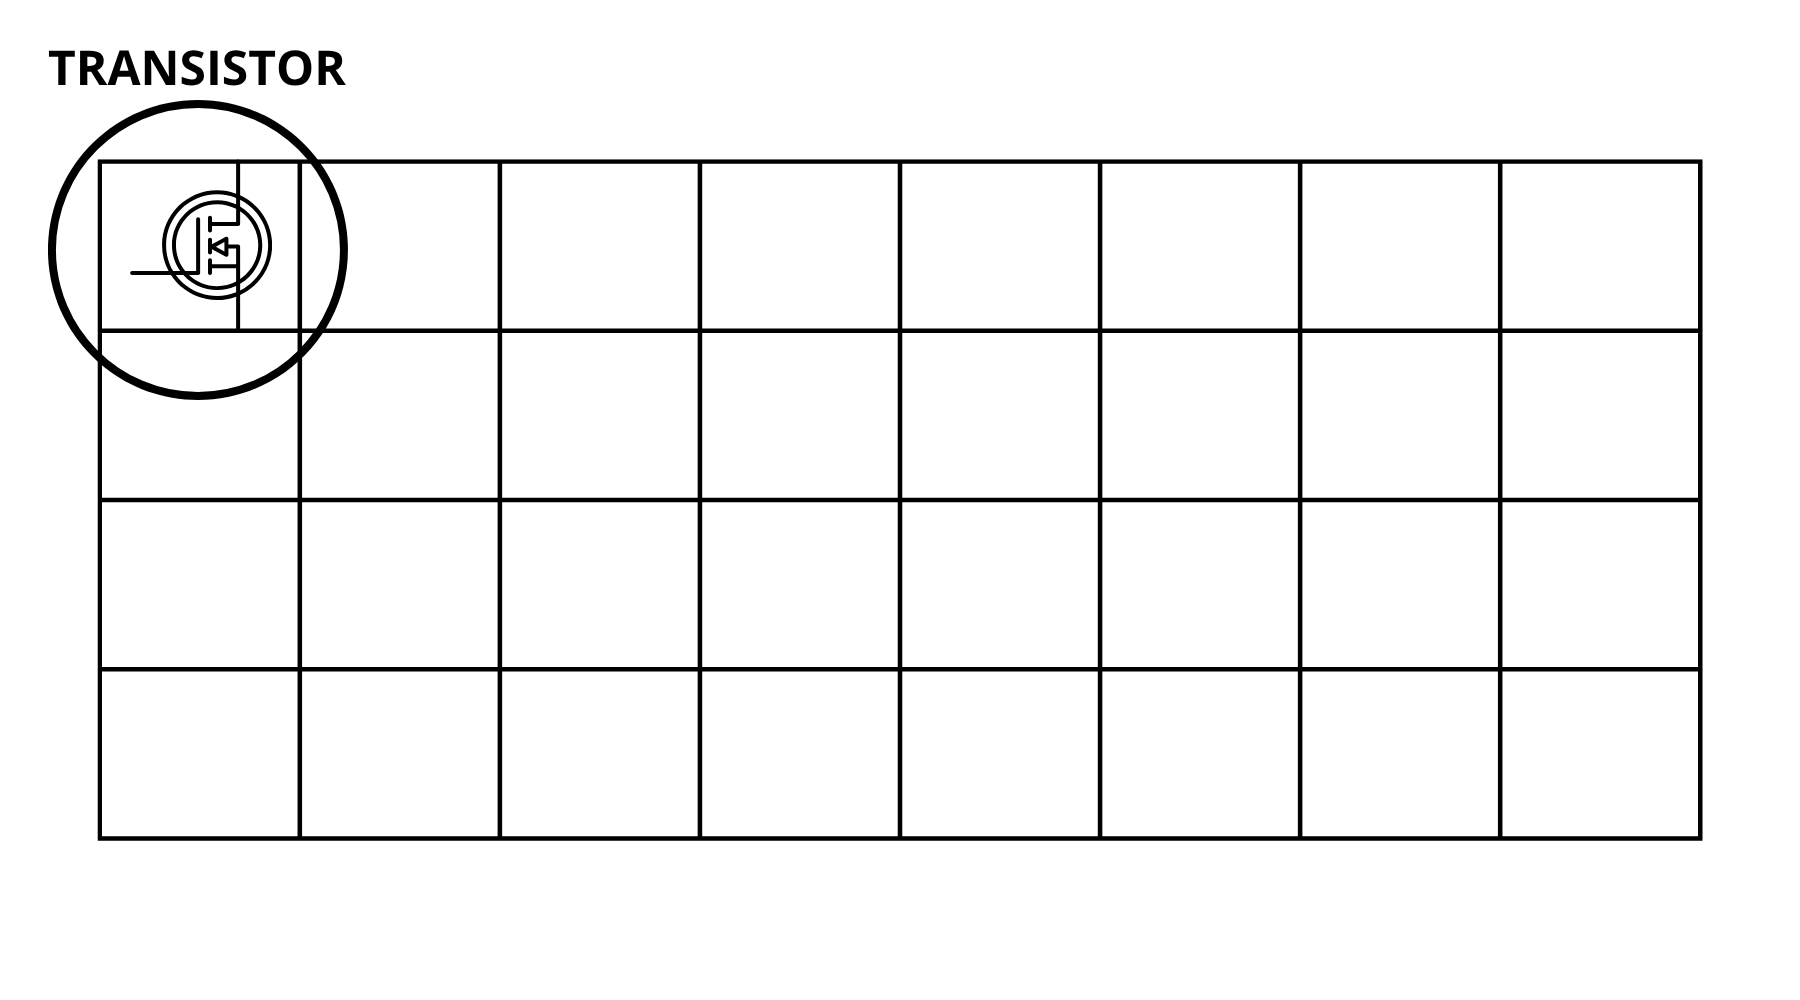
\includegraphics[width=\linewidth]{img/3.png}
        \caption{{creata con \href{www.canva.com}{Canva}}}
    \end{figure}}
\end{frame}

\begin{frame}{MEMORIA E BINARIO}
    \only<1 | handout:1>{\begin{figure}
        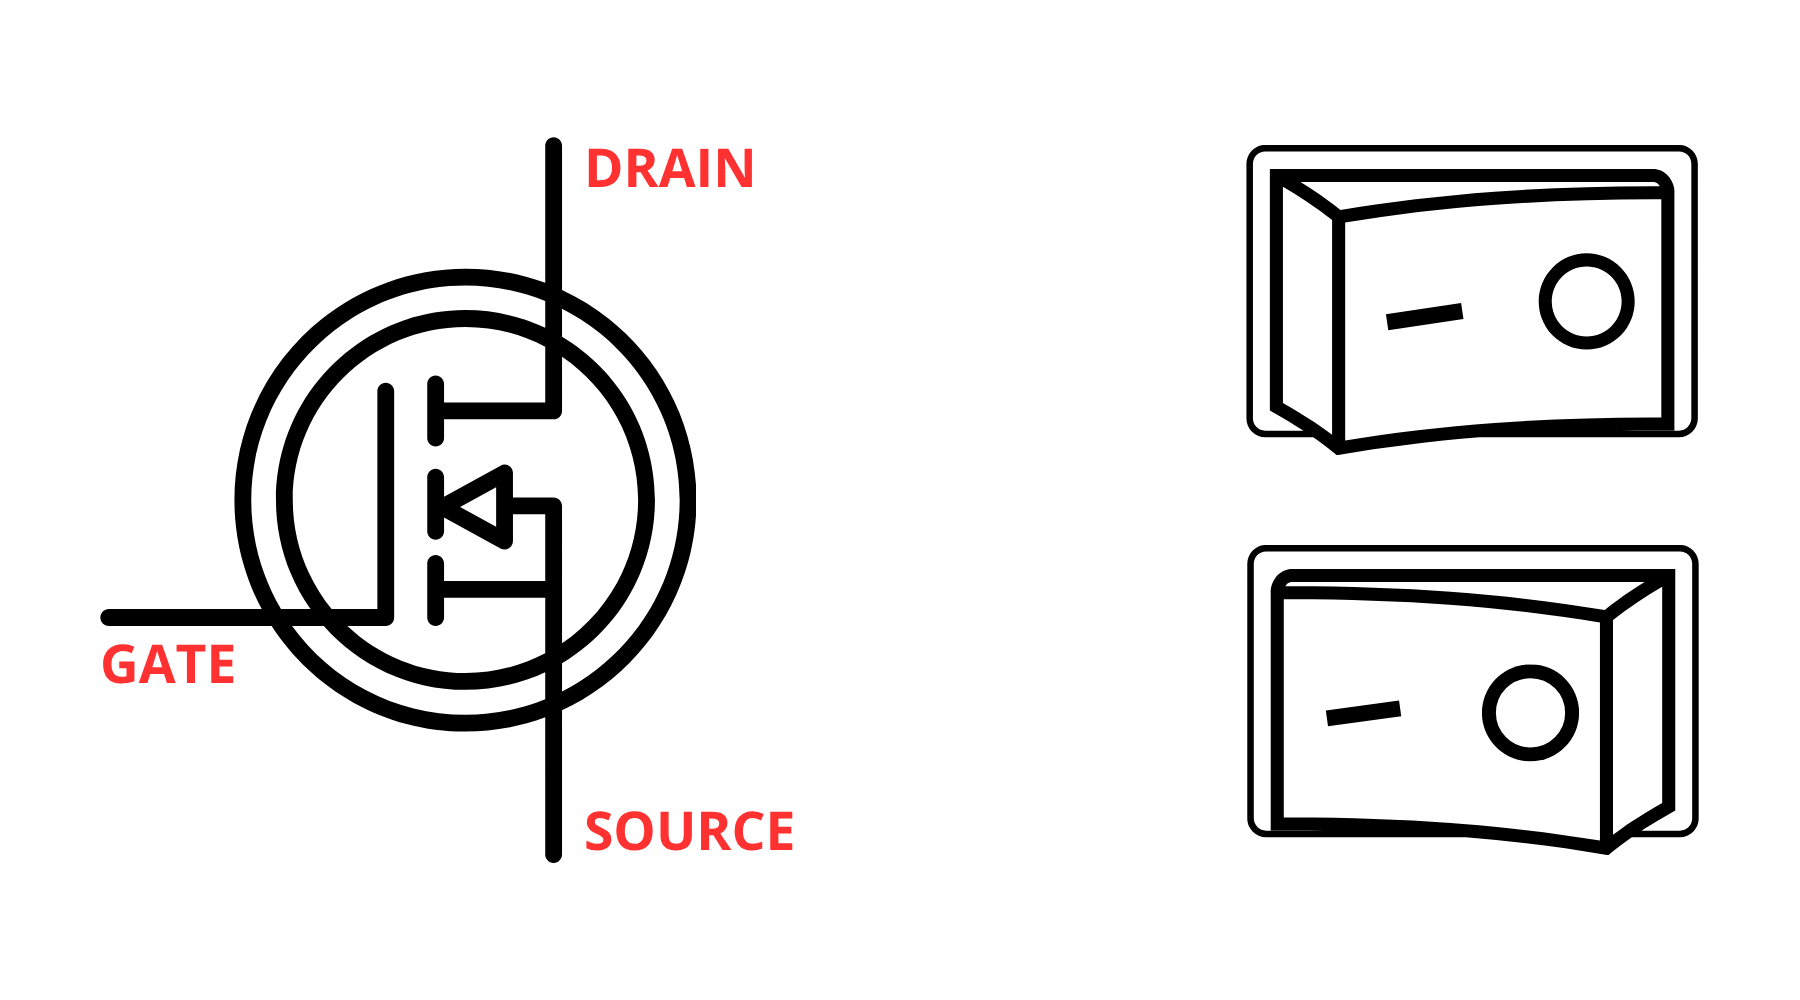
\includegraphics[width=\linewidth]{img/5.png}
        \caption{{creata con \href{www.canva.com}{Canva}}}
    \end{figure}}
    \only<2 | handout:2>{\begin{figure}
        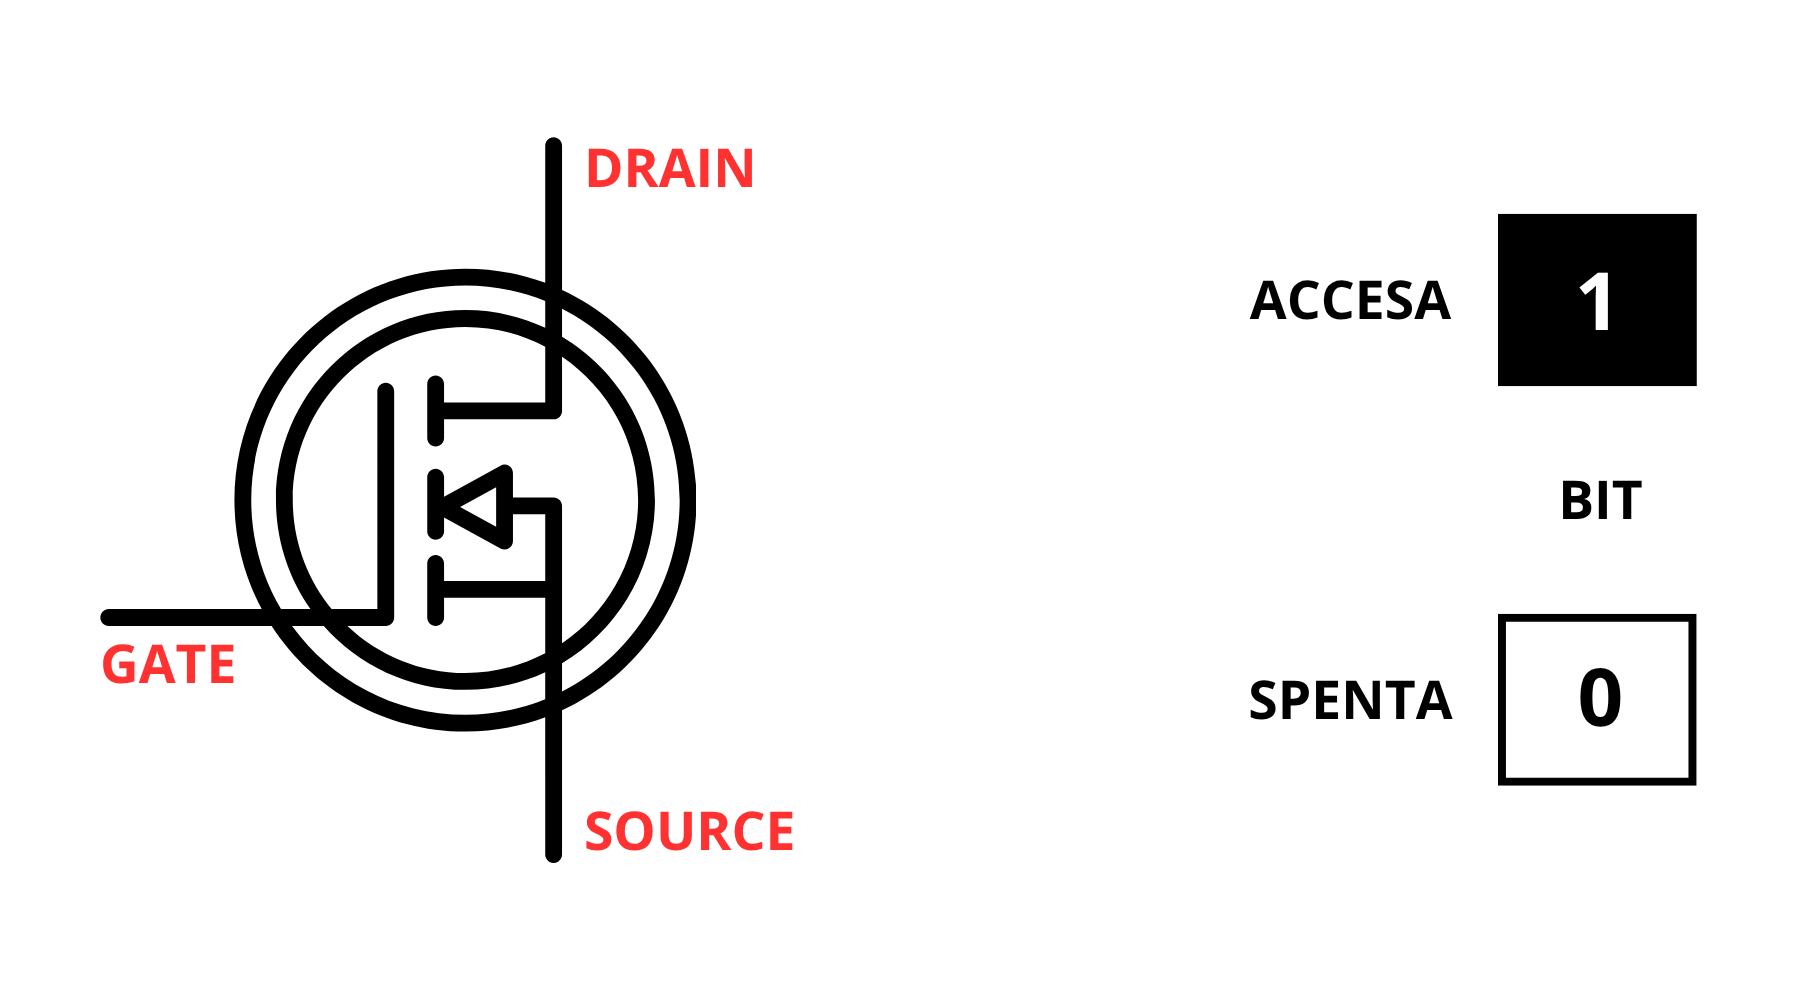
\includegraphics[width=\linewidth]{img/6.png}
        \caption{{creata con \href{www.canva.com}{Canva}}}
    \end{figure}}
\end{frame}

\begin{frame}{MEMORIA E BINARIO}
    \only<1 | handout:1>{\begin{figure}
        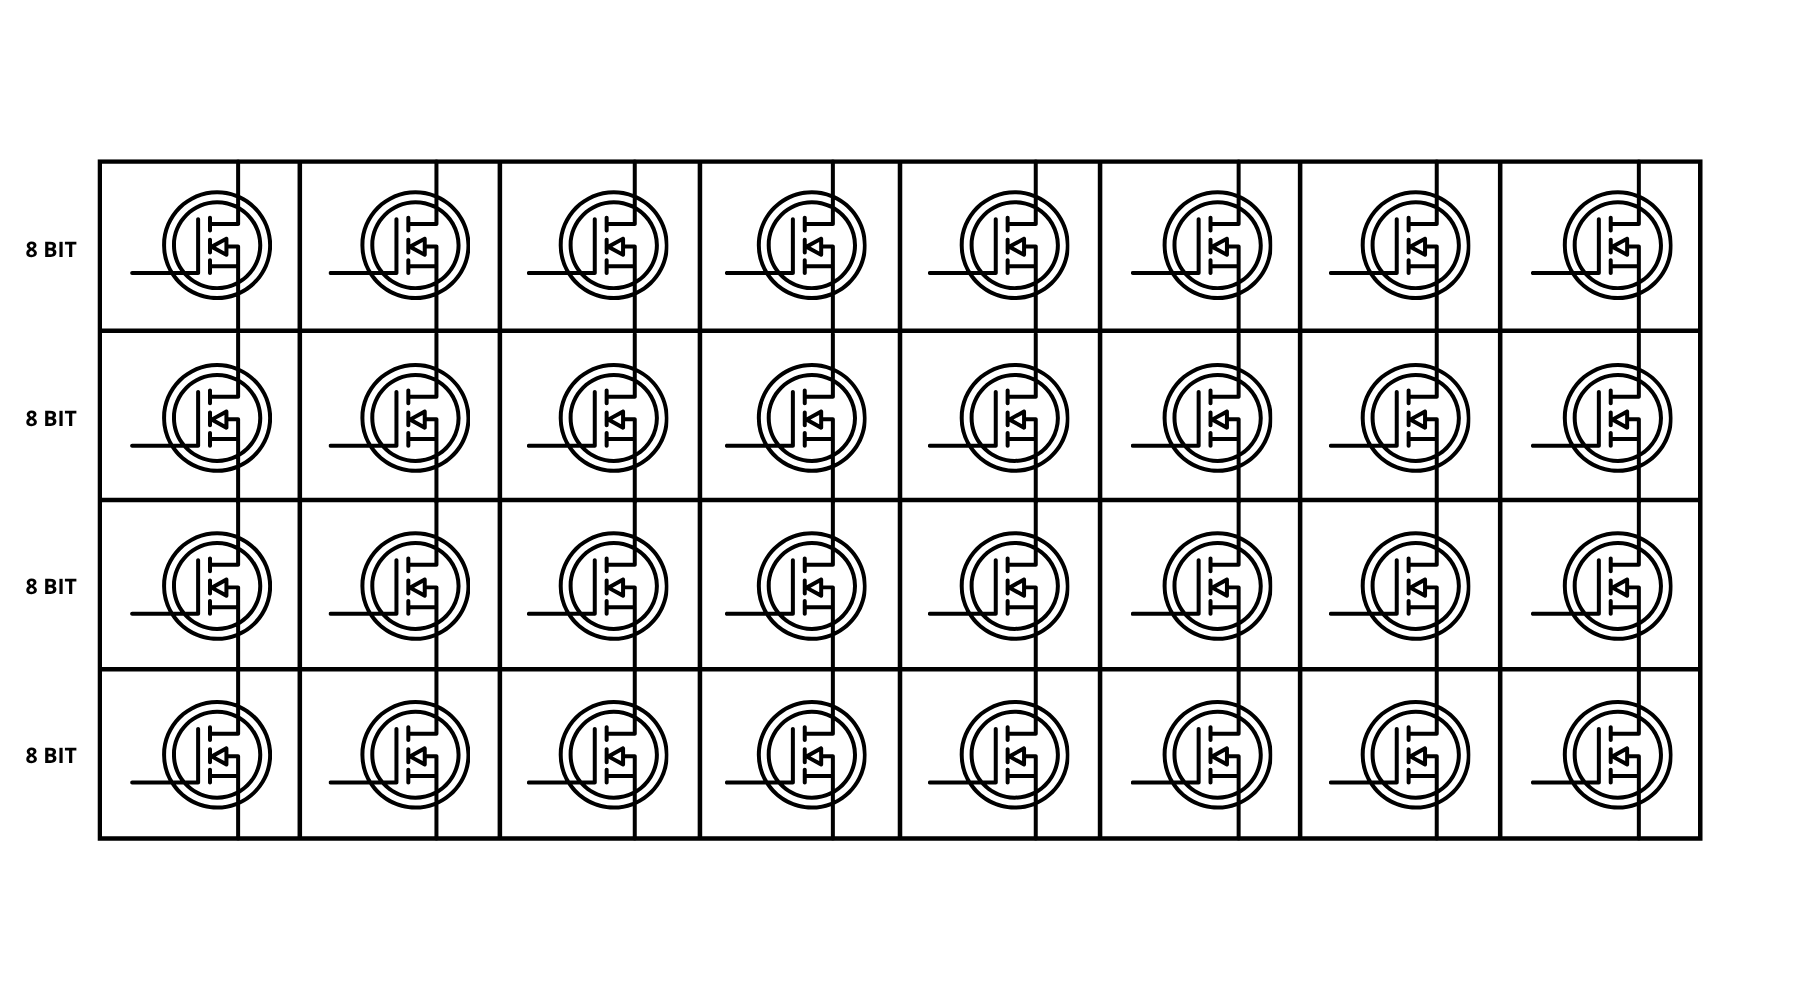
\includegraphics[width=\linewidth]{img/7.png}
        \caption{{creata con \href{www.canva.com}{Canva}}}
    \end{figure}}
    \only<2 | handout:0>{\begin{figure}
        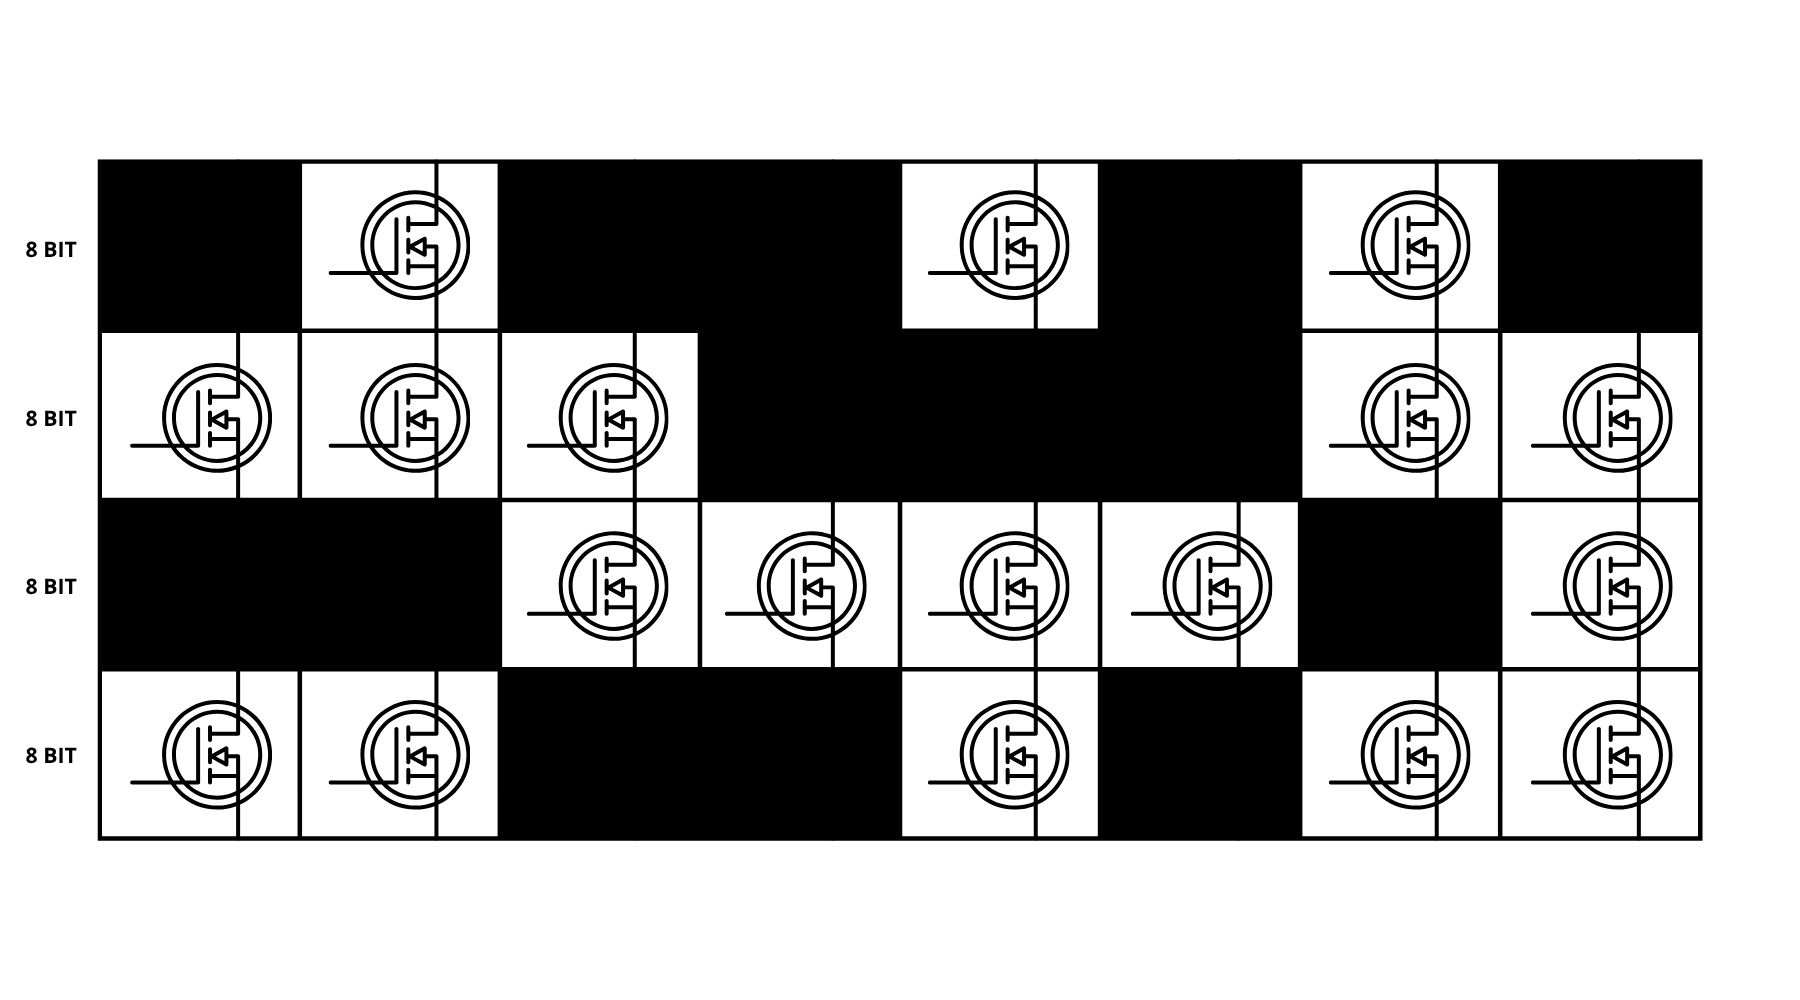
\includegraphics[width=\linewidth]{img/8.png}
        \caption{{creata con \href{www.canva.com}{Canva}}}
    \end{figure}}
    \only<3 | handout:0>{\begin{figure}
        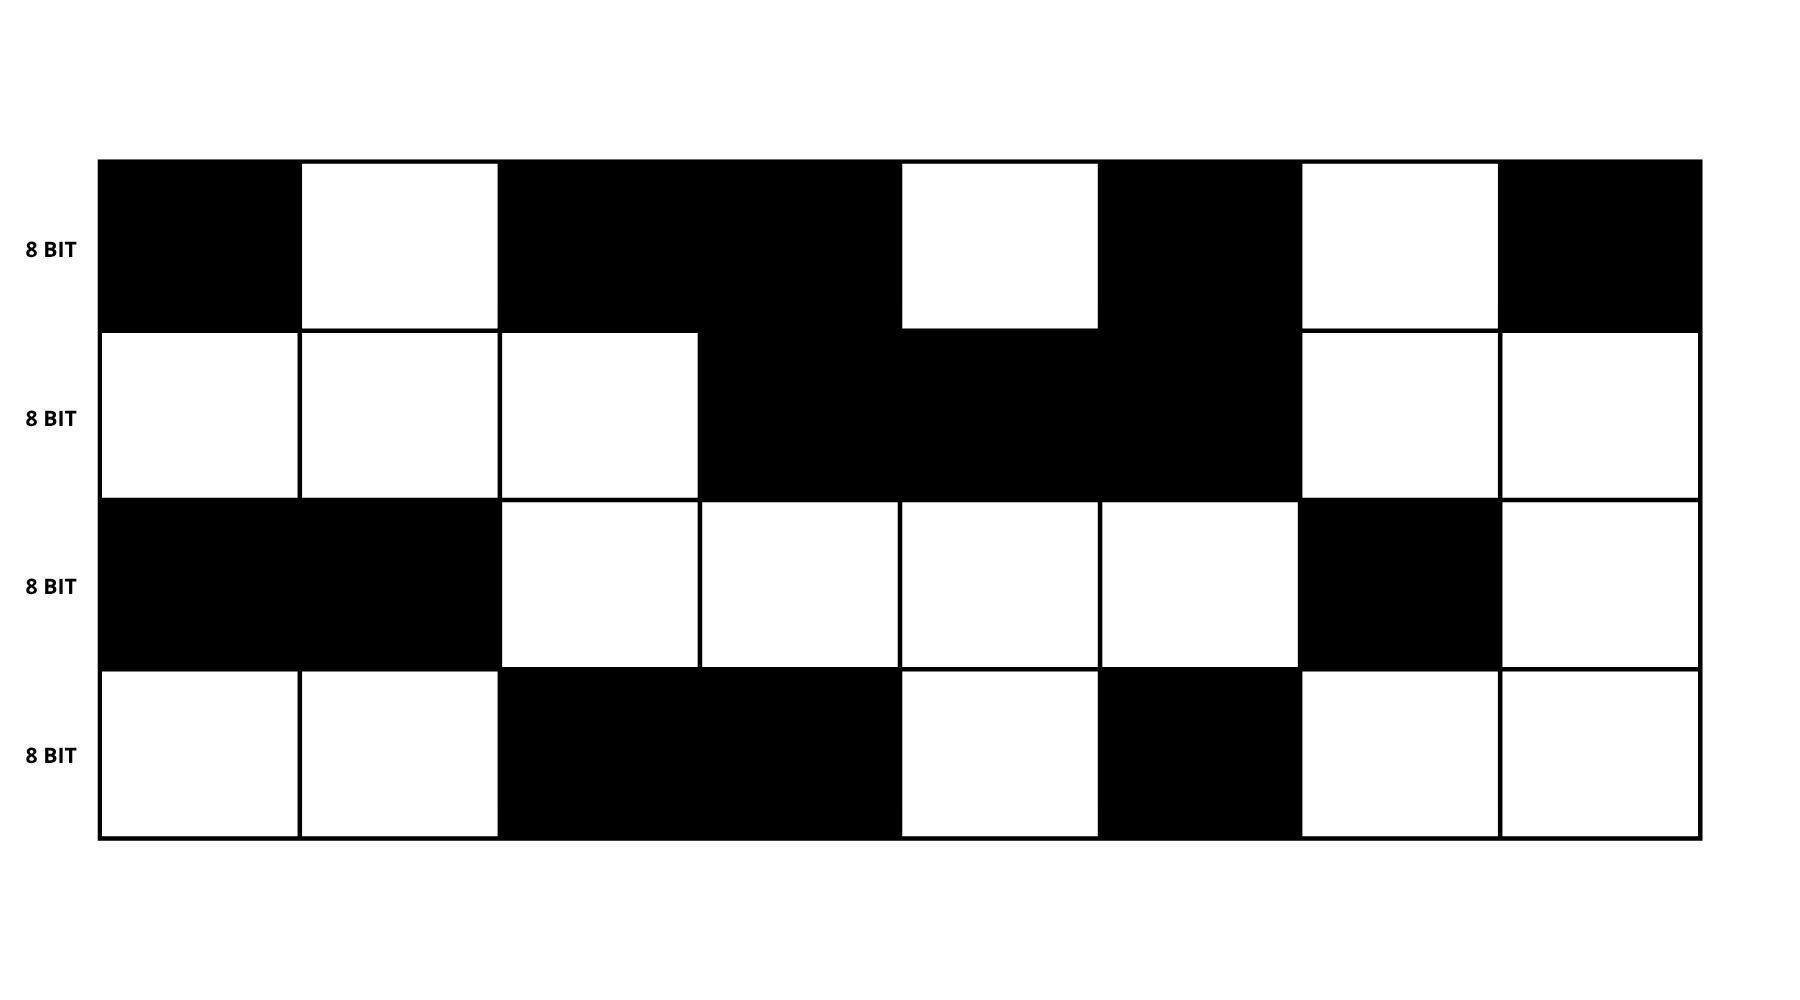
\includegraphics[width=\linewidth]{img/9.png}
        \caption{{creata con \href{www.canva.com}{Canva}}}
    \end{figure}}
    \only<4 | handout:2>{\begin{figure}
        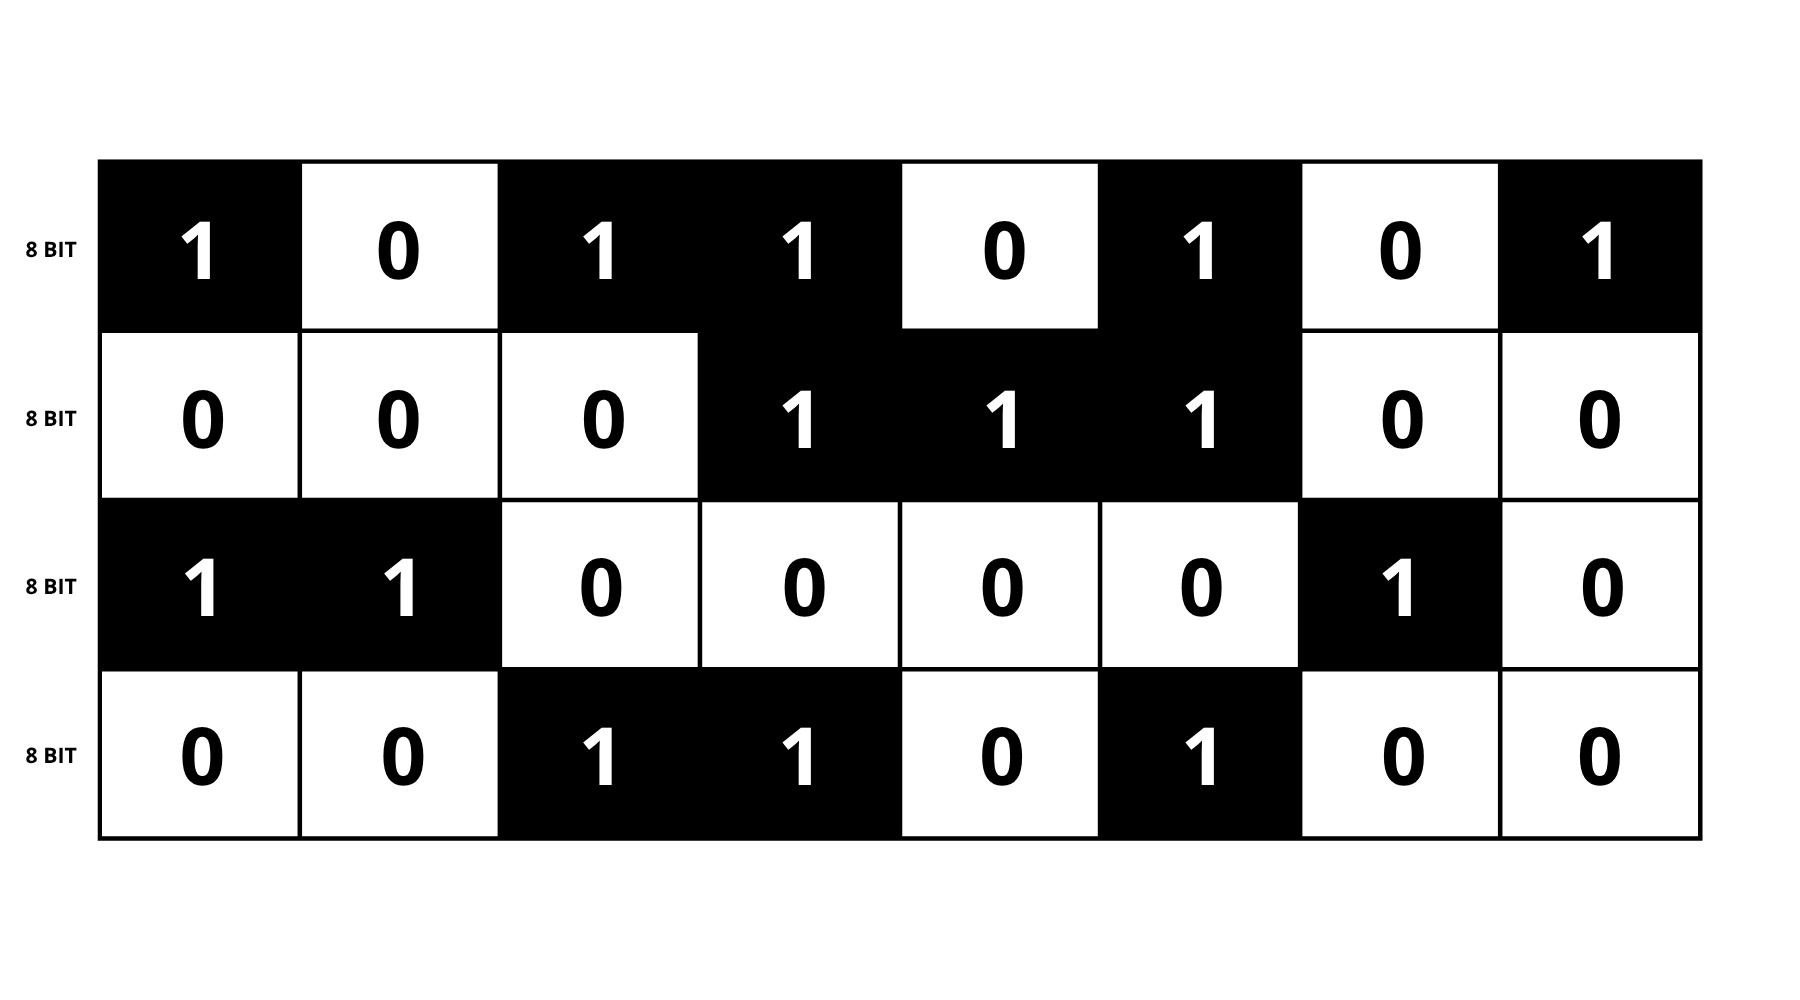
\includegraphics[width=\linewidth]{img/10.png}
        \caption{{creata con \href{www.canva.com}{Canva}}}
    \end{figure}}
\end{frame}

\begin{frame}{MEMORIA E BINARIO}
    \only<1 | handout:0>{\begin{figure}
        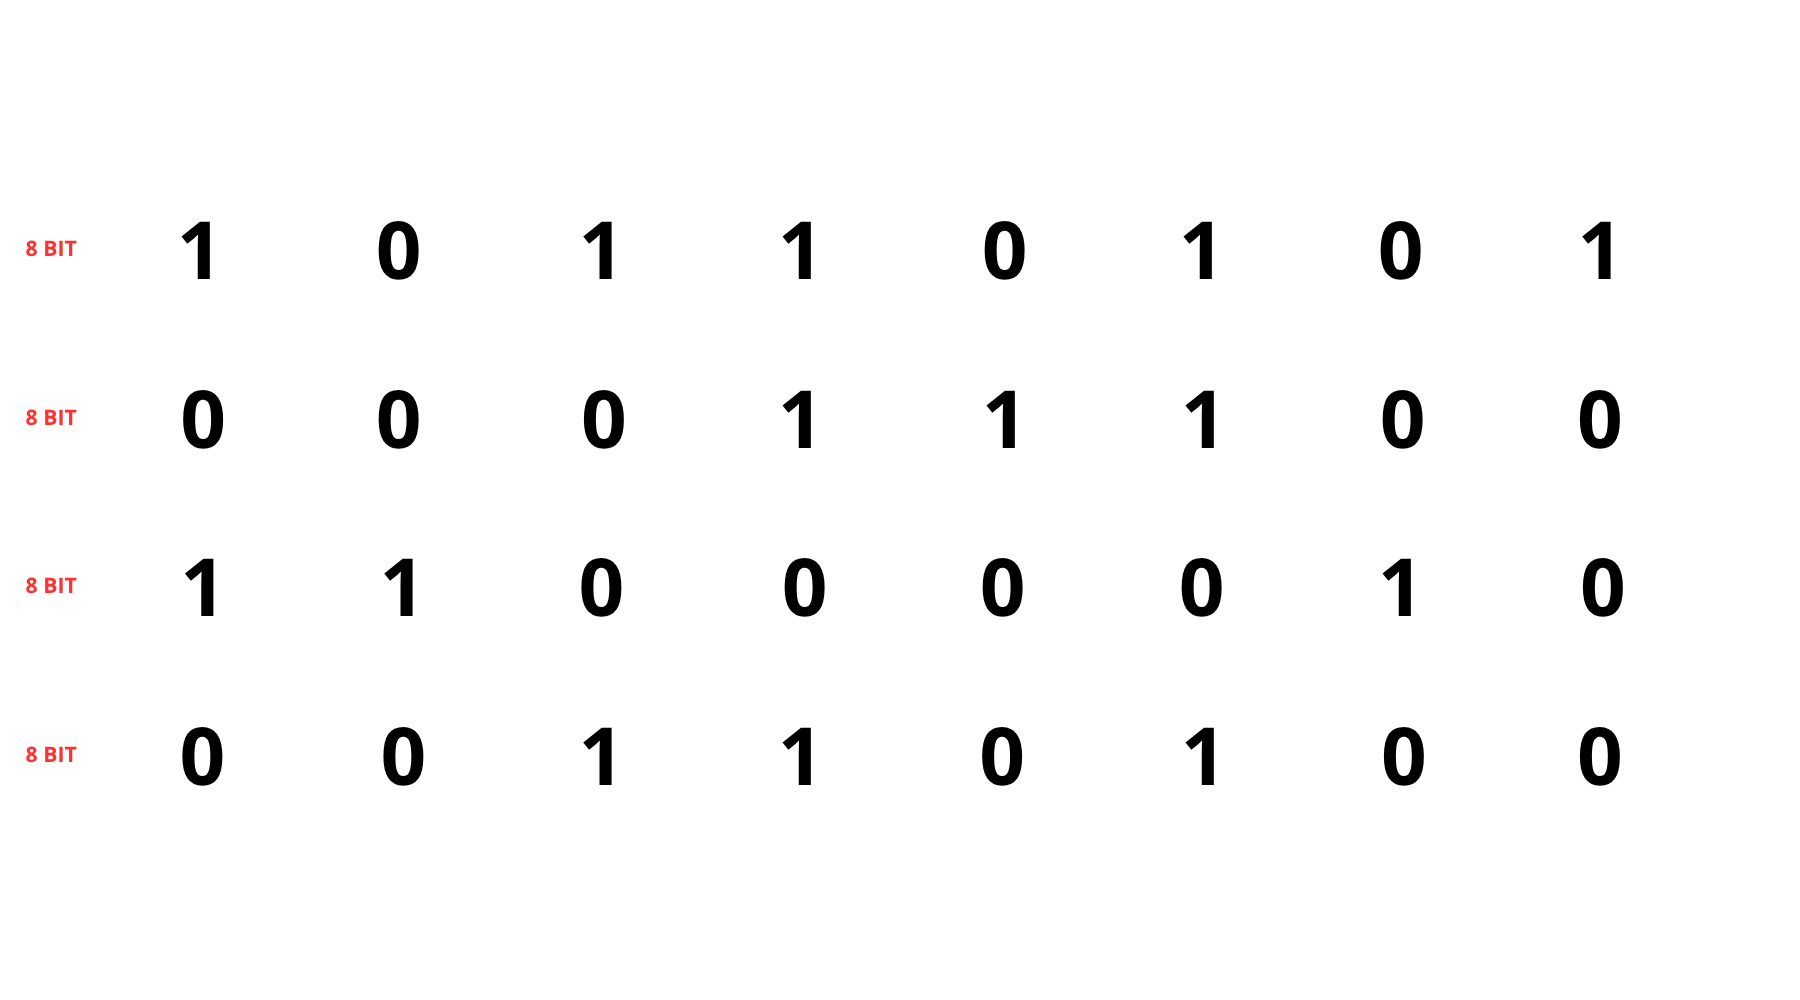
\includegraphics[width=\linewidth]{img/11.png}
        \caption{{creata con \href{www.canva.com}{Canva}}}
    \end{figure}}
    \only<2 | handout:0>{\begin{figure}
        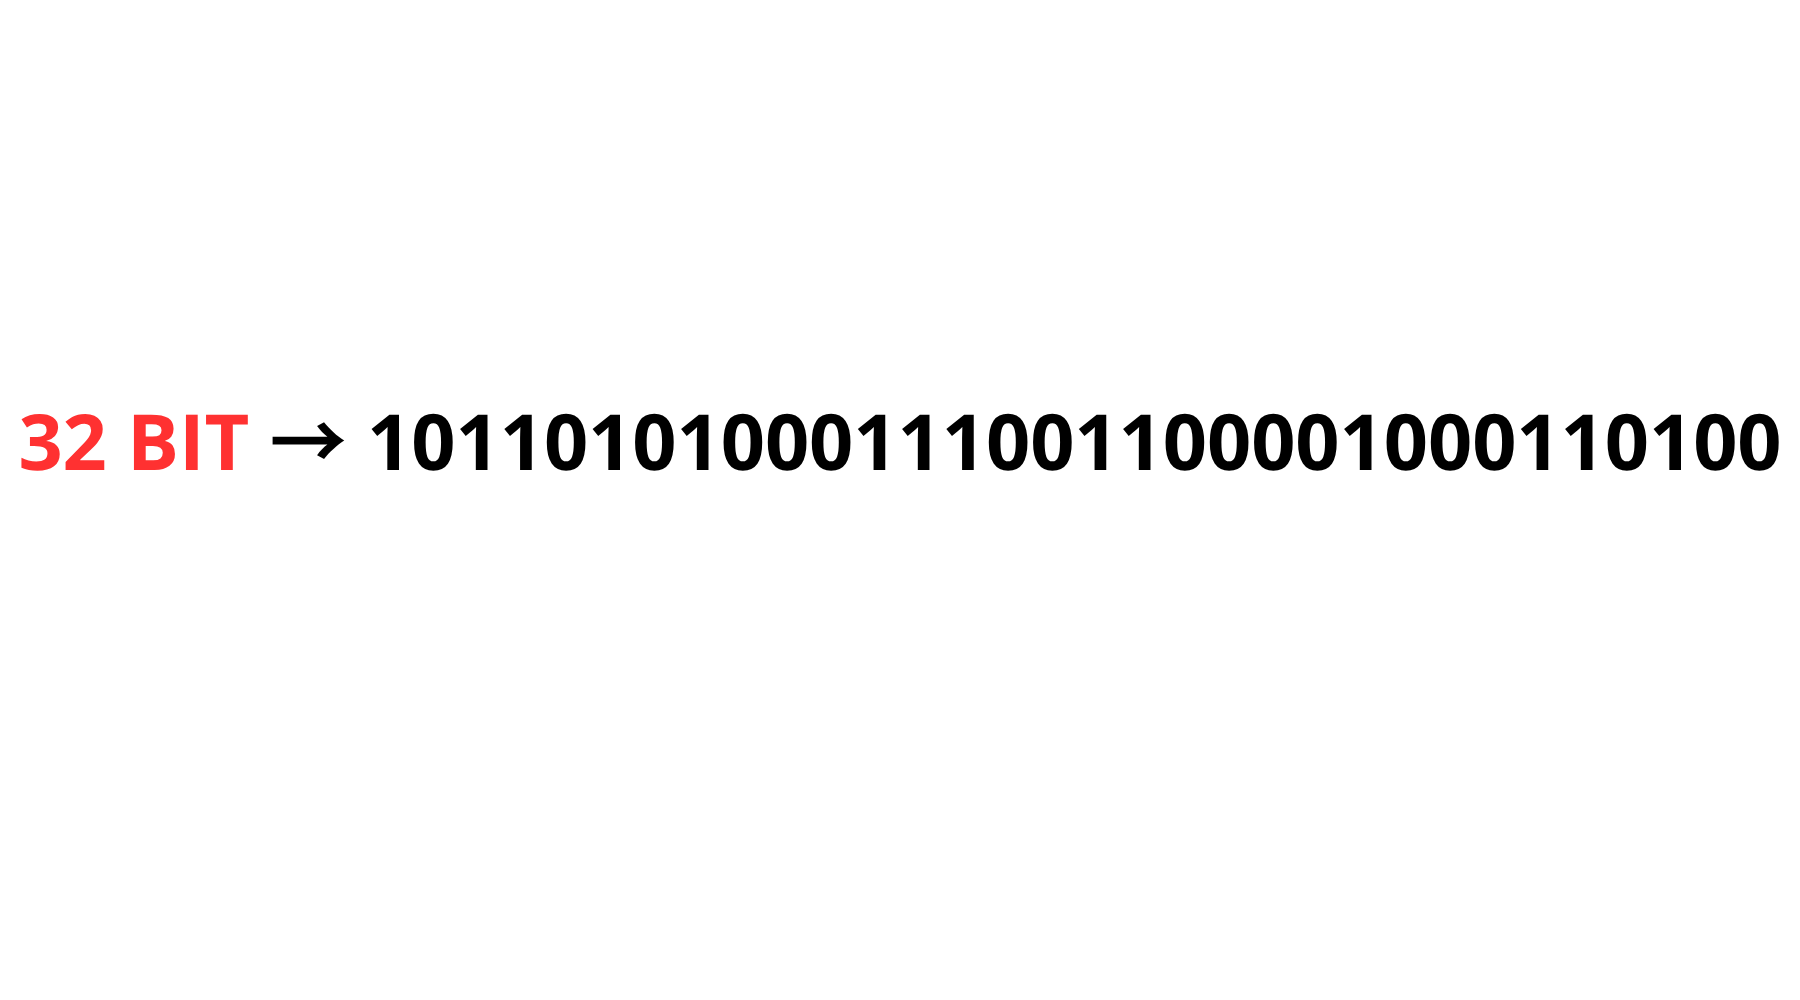
\includegraphics[width=\linewidth]{img/12.png}
        \caption{{creata con \href{www.canva.com}{Canva}}}
    \end{figure}}
    \only<3 | handout:1>{\begin{figure}
        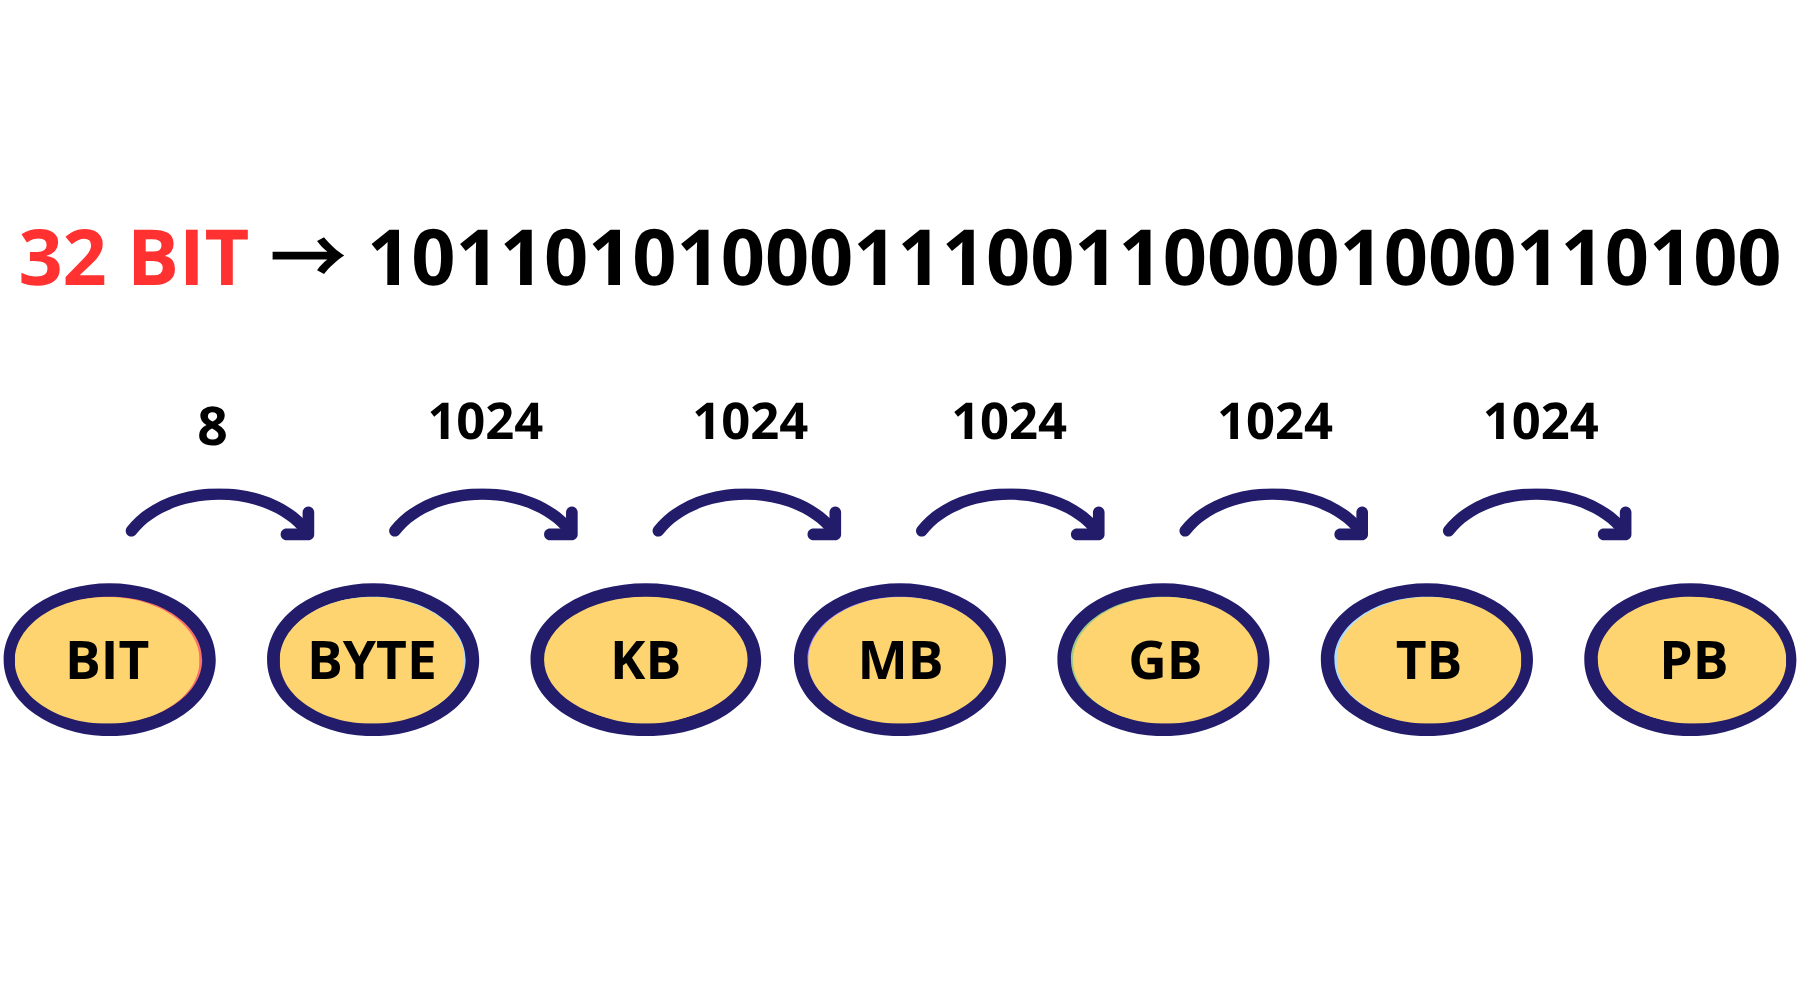
\includegraphics[width=\linewidth]{img/13.png}
        \caption{{creata con \href{www.canva.com}{Canva}}}
    \end{figure}}
\end{frame}

\end{document}